\textcolor{blue}{Problem 5}

5.4 Huffman coding. Consider the random variable

$$\left.X=\left(\begin{array}{ccccccc}x_1&x_2&x_3&x_4&x_5&x_6&x_7\\0.49&0.26&0.12&0.04&0.04&0.03&0.02\end{array}\right.\right).$$

(a) Find a binary Huffman code for $X$.

(b) Find the expected code length for this encoding.

(c) Find a ternary Huffman code for $X.$

\textcolor{blue}{Solution}

(a) The binary Huffman tree and the corresponding binary Huffman code for $X$ are shown below.
\begin{figure}[htbp]
    \centering
	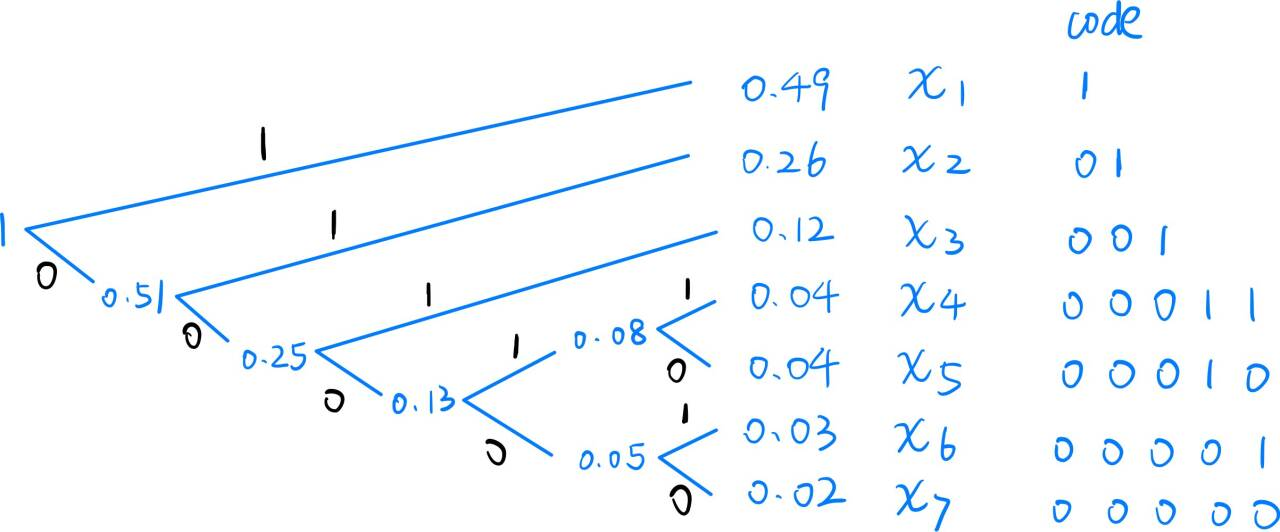
\includegraphics[width=0.66\textwidth]{../binary_Huffman_coding.png}
\end{figure}

(b) The length of the binary Huffman code for $x_i$ is $l(x_i)$:

\begin{table*}[!htbp]
\centering
\begin{tabular}{c|ccccccc}
$x_i$ & $x_1$ & $x_2$ & $x_3$ & $x_4$ & $x_5$ & $x_6$ & $x_7$ \\
\hline
$l(x_i)$ & $1$ & $2$ & $3$ & $5$ & $5$ & $5$ & $5$
\end{tabular}
\end{table*}

So the expected code length for this encoding is
$$\bar{L}=\sum_{i=1}^tp(x_i)l(x_i)=2.02\text{\ bits}$$

(c) The ternary Huffman tree and the corresponding ternary Huffman code for $X$ are shown below.
\begin{figure}[htbp]
    \centering
	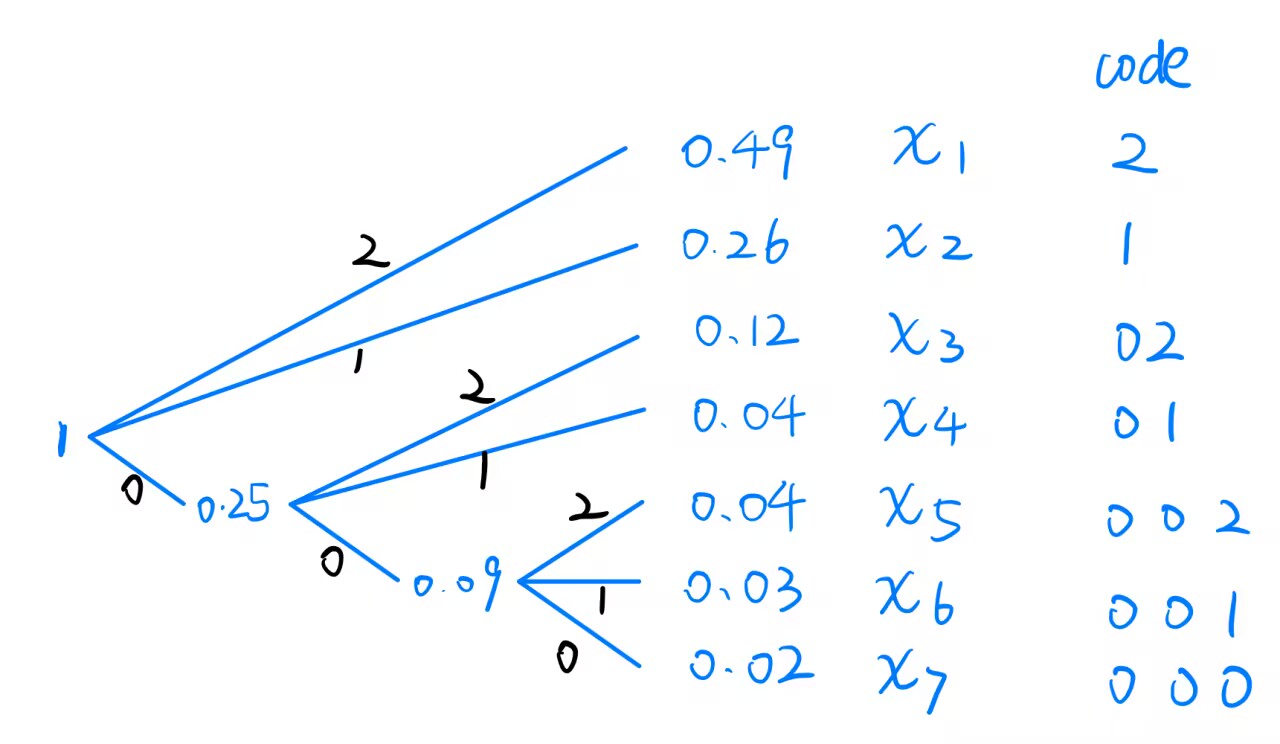
\includegraphics[width=0.66\textwidth]{../ternary_Huffman_coding.png}
\end{figure}

\newpage